% Chapter 6

\chapter{Despliegue}
\label{capitulo6}

\section{Plan de Despliegue}
En el curso del desarrollo, depuración y ejecución de pruebas llegó a ser evidente en enorme consumo de recursos necesarios para levantar todos los servicios desarrollados y auxiliares a la vez, razón por el cual, se ha visto la necesidad de un rediseño de forma mas liviana de la manera en que se despliegue todos los componentes integrados a la aplicación para con ello terminar las fases mencionadas anteriormente y dar paso a ejecución en ambientes de pocos recursos, tanto en el ámbito de desarrollo como de producción. En la implementación original de la arquitectura física para el desarrollo, se había planteado una colección de maquinas virtuales quienes representarían servidores distintas dentro de una red, pero para temas de optimizar recursos, se ha realizado los siguientes cambios los cuales se documentan a lo largo de este capitulo:
\begin{itemize}
	\index{Kubernetes}
	\item Kubernetes (backend de virtualización) se ubica en una maquina virtual de Xen (con paravirtualización activa para aumentar el rendimiento del sistema virtualizado) dado que el mismo, por temas de seguridad, debe seguir de una forma aislada. De esta forma se simula que esta en un servidor aparte, sea físico o virtual (se recomienda mejor virtualizar todo el cluster final de Kubernetes en algún hipervisor de tipo 1 para garantizar mayor seguridad y aislamiento) pero sin la mayor parte de las perdidas de rendimiento que se dio con MiniKube (alojado en VirtualBox).
    \index{Docker}
    \item Los servicios auxiliares en lugar de ser maquinas virtuales de Xen ahora son contenedores de Docker.
    \index{SystemD}
    \item Los servicios desarrollados se los han convertido en servicios (Systemd) del sistema operativo, no tanto por temas de rendimiento (aunque se podría mejorar el rendimiento de esta forma, asignándoles a un usuario con mayor prioridad de ejecución como el usuario root\footnote{Pero realizarlo esta afuera del alcance de este tesis, una solución así de software tampoco puede cambiar los recursos físicos de la maquina.}\footnote{Nunca se debe asignar un servicio que se consume en la red externa a algún usuario con privilegios de superusuario, como root, ya que el mismo abre todo el sistema operativo a un nuevo vector de ataque por el mismo servicio. En este caso debe ser un nuevo usuario, preferiblemente uno por cada servicio, con acceso restringido que tiene mayor prioridad de ejecución para sus procesos.}) si no por temas de facilitar la administración del mismo.
    \index{NGinX}
    \item La integración de los servicios con NGinX para que el mismo puede protegerlos y operar en la capacidad de proxy inversa, proxy de terminación SSL/TLS, servidor de archivos estáticos y validador de peticiones sin mayor perdida de rendimiento.
\end{itemize}
% TODO: diagrama de red/fisica

\section{Preparaciones del Ambiente de Despliegue}
Para preparar el ambiente de despliegue se lo ve pertinente planificar direcciones IP, dominios y puertos para los varios servicios que requieren ser levantados:
\begin{description}
	\item[Maquina Física] con Debian 9.x para Servicios y Docker: \textit{10.10.10.1}
    \begin{description}
    	\item[NGinX] \textit{http://0.0.0.0:80} \index{NGinX}
        \begin{itemize}
            \item \textit{http://10.10.10.1:80} \& \textit{http://git.localhost:80} -> GitWeb (HTTP)
            \item \textit{http://gitedu.localhost:80} -> GitEDU (HTTP)
            \item \textit{http://edunube.localhost:80} -> EduNube (HTTP)
            \item \textit{http://gitsrvendpoint.localhost:80} -> GitServerHTTPEndpoint (HTTP)
            \item \textit{http://gitlab.localhost:80} -> GitLab (HTTP)
            \item \textit{http://moodle.localhost:80} -> Moodle (HTTP)
            \item \textit{http://registry.localhost:80} -> Registry (HTTP)
        \end{itemize}
        \item[GitEDU] \textit{http://0.0.0.0:8000}
        \item[EduNube] \textit{http://0.0.0.0:8010}\footnote{Previamente el puerto asignado fue :8001, pero esto estaba en conflicto con el Dashboard/Proxy de Kubernetes, por lo tanto se ha cambiado este servicio al puerto :8010}
        \item[GitServerHTTPEndpoint] \textit{http://0.0.0.0:8020}\footnote{Para temas de consistencia con el cambio de puerto de EduNube, se ha cambiado el numero de puerto de :8002 a :8020}
        \item[Kubernetes Proxy] \textit{http://0.0.0.0:8001}
        \item[Docker] \textit{10.10.10.1}
        \begin{description}
        	\item[MySQL] \textit{0.0.0.0:3306} -> \textit{moodledb:3306} (TCP/MySQL)
        	\item[Moodle] \textit{0.0.0.0:8201} -> \textit{moodle:80} (HTTP)
        	\item[GitLab CE] \textit{10.10.10.1}
            \begin{itemize}
            	\item \textit{0.0.0.0:8143} -> \textit{gitlab:443} (HTTPS)
            	\item \textit{0.0.0.0:8101} -> \textit{gitlab:80} (HTTP)
            	\item \textit{0.0.0.0:8122} -> \textit{gitlab:22} (SSH)
            \end{itemize}
            \item[Registry] \textit{0.0.0.0:5000} -> \textit{registry:5000} (HTTP)
        \end{description}
    \end{description}
    \item[Maquina Virtual (Xen)] con Debian 9.x para el Cluster (solo 1 nodo maestro) de Kubernetes: \textit{10.10.10.12}
\end{description}

\subsubsection{Moodle en Docker}
La instalación de Moodle en Docker consiste de los siguientes pasos:
\begin{enumerate}
	\item Bajar el imagen de Docker oficial de MySQL:
    \begin{lstlisting}    
docker pull mysql
    \end{lstlisting}
    \item Bajar un imagen de Docker de Moodle:
    \begin{lstlisting}    
docker pull jauer/moodle
    \end{lstlisting}
    \item Ejecutar el imagen de MySQL en el fondo (-d) con un nombre posible de identificar (moodledb), paso de puertos (10.10.10.1:3306 -> moodledb:3306), un volumen de persistencia para el motor de base de datos, nombres de bases de datos, usuarios y contraseñas de MySQL y una petición de que siempre se reinicia el contenedor a lo que muere con algún error:
    \begin{lstlisting}    
docker run -d --name moodledb -p 3306:3306 -v \
/srv/moodle/mysql:/var/lib/mysql -e \
MYSQL_DATABASE=moodle -e MYSQL_ROOT_PASSWORD=moodle \
-e MYSQL_USER=moodle -e MYSQL_PASSWORD=moodle \
--restart always mysql
    \end{lstlisting}
    \item Ejecutar el imagen de Moodle con opciones similares al anterior, con un enlace a la base de datos con un dominio local de DB, metadatos del url en que debe responder y ocupar el puerto 8201 local como puerto 80 del contenedor (un passthrough):
    \begin{lstlisting}    
docker run -d -P --name moodle --link moodledb:DB\
-e MOODLE_URL=http://10.10.10.1:8201 -p 8201:80 \
-v /srv/moodle/data:/var/moodledata \
--restart always jhardison/moodle
    \end{lstlisting}
    \item Y finalmente visitamos http://10.10.10.1:8201/ para terminar la instalación inicial de Moodle y realizar su configuración inicial.
\end{enumerate}

\subsubsection{GitLab en Docker}
Para instalar GitLab en Docker\citep{GitLab-Docker-Images}, se sigue pasos similares a los vistos previamente con Moodle:
\begin{enumerate}
	\item Bajar el imagen de Docker:
    \begin{lstlisting}    
docker pull gitlab/gitlab-ce
    \end{lstlisting}
    \item Ejecutar el imagen de Docker:
    \begin{lstlisting}    
docker run --detach --hostname 10.10.10.1 \
--publish 8143:443 --publish 8101:80 \
--publish 8122:22 --name gitlab --restart always \
--volume /srv/gitlab/config:/etc/gitlab \
--volume /srv/gitlab/logs:/var/log/gitlab \
--volume /srv/gitlab/data:/var/opt/gitlab \
gitlab/gitlab-ce:latest
    \end{lstlisting}
    \item Visitar http://10.10.10.1:8101/ para cambiar la contraseña de root
\end{enumerate}

\subsubsection{Registry en Docker}
A diferencia de el ambiente de desarrollo, que ocupa el Docker Registry de GitLab\footnote{Se puede encontrar en \url{https://gitlab.com/nishedcob/GitEDU/container\_registry}}, para el ambiente de despliegue se plantea replicar el servicio de forma local para reducir el consumo de red. Para ello, se utiliza un contenedor de Docker:
\begin{enumerate}
	\item Bajar el imagen de Docker:
    \begin{lstlisting}
docker pull registry
    \end{lstlisting}
    \item Ejecutar el imagen de Docker:
    \begin{lstlisting}
docker run -d -p 5000:5000 --restart always \
--name registry registry
    \end{lstlisting}
\end{enumerate}
El proyecto de Docker, en parte por su mala fama de ser insegura, toma muy enserio la seguridad. Por lo tanto, aunque se puede consumir normalmente un Docker Registry por HTTP con el dominio localhost, al ocupar cualquier otro dominio o direccion IP, el cliente de Docker por defecto exige que las llamadas al API en el servidor sean sobre HTTPS. Con la finalidad de no complicar la configuracion más y tambien por el hecho de que la arquitectura fisica del despliegue realmente no sale del localhost, aunque para Docker le parece que si (obviamente no tiene conocimiento de son maquinas virtuales a los cuales el acceso es por adaptadores de red virtuales, etc), se ha optado para realizar la adecuada configuracion al archivo \texttt{/etc/docker/daemon.json} en cada host que consume el Registry sobre HTTP para que los mismos no exigen HTTPS donde solo existe HTTP. La configuracion es lo siguiente (en este caso no existia el archivo JSON, entonces se lo creaba con los contenidos a continuacion, en otros casos se agregaria solo los valores abajo a los valores existentes):
\begin{lstlisting}
{
          "insecure-registries" : [
                  "10.10.10.1:5000"
          ]
}
\end{lstlisting}
Despues de realizar aquello configuracion es necesario reiniciar Docker \index{Docker} para que tome en cuenta los cambios con el commando \texttt{systemctl restart docker}. Para popular el registry con los contenedores necesarias para ejecuccion de codigo con el sistema EduNube, puede referirse a los commandos encontrados en \\
\texttt{docker/commands-local-doc.sh} del repositorio principal. Este script toma los contenedores compilados previamente durante el desarrollo, los prepara para subirse y se los sube al Registry para que otros consumidores del mismo Registry tengan acceso a ellos.

\index{Hipervisor} \index{Virtualización} \index{Contenedor} \index{Xen}
\subsubsection{Máquina Virtual de Xen}
Con el fin de proteger la maquina física contra usuarios finales, sean maliciosos o solo sin conocimientos adecuados, hay la necesidad de que el ambiente que ejecuta código sea aislado con virtualización. Pero el rendimiento de esta maquina virtual necesita ser maximizada para poder permitir su uso con un mínimo de recursos. Es, por lo tanto, que se ha propuesta utilizar una maquina virtual de Xen de baja nivel con mejores de rendimiento con la tecnología de paravirtualización con la finalidad de que esta misma logra ofrecer alta aislamiento, y por lo tanto seguridad, frente una alta rendimiento.

\index{Kubernetes}
\paragraph{Construcción de Servidor Virtualizado para Cluster de Kubernetes}
Las características mínimas que pide Kubernetes para su nodo maestro son 2 núcleos y 2 GiB de RAM, es por aquello razón que se crea una maquina virtual paravirtualización con estas mismas características. En el curso del año que se ha trabajado este trabajo de titulación la comunidad de Debian se ha logrado arreglar  el bug que antes causó problemas la ultima vez que se realizó una maquina virtual nueva de Debian 9 y es con este motivo que se puede crear una maquina virtual nueva sin ninguna necesidad para pasos adicionales, los resultados de la creacion del mismo, se indica en la figura \ref{fig:create-k8s-xen-vm}:
\begin{lstlisting}
xen-create-image --hostname=debian-k8s-master \
--ip=10.10.10.12 --netmask=255.255.255.0 \
--gateway=10.10.10.1 --memory=2048mb --vcpus=2 \
--lvm=Xephyr-VG --pygrub --dist=stretch --force \
--size=10240mb --swap=1024mb
\end{lstlisting}
\begin{figure}
	\begin{center}
		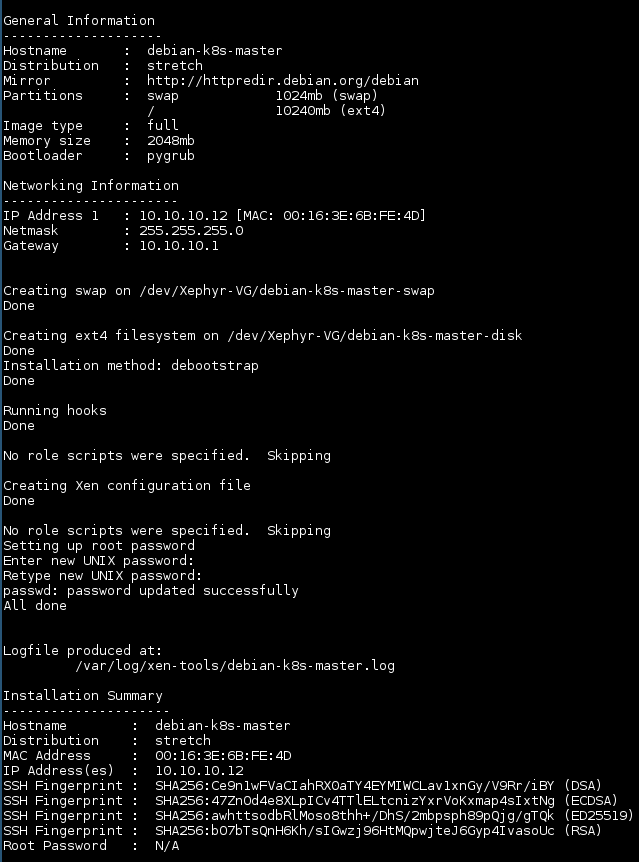
\includegraphics[width=0.5\textwidth]{Figures/create-k8s-vm.png}
	\end{center}
    \caption{Resultados de Crear la Maquina Virtual de Xen para el Cluster de Kubernetes de un solo Nodo}
    \label{fig:create-k8s-xen-vm}
\end{figure}

\index{Docker}
\paragraph{Instalación de Docker}
Para utilizar Kubernetes dentro de esta maquina virtual es necesario primero contarnos con una instalación de Docker. Kubernetes no garantiza que va a funcionar con las ultimas versiones de Docker ya que el API de Docker cambia constantemente, especialmente con actualizaciones de seguridad, pero de esta misma forma para la seguridad de la misma, queremos contar con la misma forma estable. Se instala de la siguiente manera en Debian (para otros sistemas operativos, a lo mucho solo se tendría que cambiar el gestor de paquetes apt por el respectivo de su sistema):
\begin{enumerate}
	\item Actualizar el sistema operativo
    \begin{lstlisting}
apt update
apt upgrade
    \end{lstlisting}
    \item Instalar curl si es que no esta instalado previamente
    \begin{lstlisting}
apt install curl
    \end{lstlisting}
    \item Bajar el instalador actual de Docker
    \begin{lstlisting}
curl -fsSL get.docker.com -o get-docker.sh
    \end{lstlisting}
    \item Ejecutar el instalador de Docker
    \begin{lstlisting}
sh get-docker.sh
    \end{lstlisting}
\end{enumerate}
% TODO: include Screenshot_2017-12-29_15-31-49.png

Para utilizar el Registry creado anteriormente, se agrega el siguiente configuracion a las maquinas del cluster (seguido por el reinicio del servicio de Docker con \texttt{systemctl restart docker}):
\begin{lstlisting}
{
          "insecure-registries" : [
                  "10.10.10.1:5000"
          ]
}
\end{lstlisting}

\index{Kubernetes}
\paragraph{Instalación de Cluster de Kubernetes}
Para instalar el cluster de Kubernetes, el proceso es relativamente sencillo con una herramienta que se llama \texttt{kubeadm} que se encarga de levantar, gestionar y bajar nodos del cluster. Primero para instalar el mismo:
\begin{enumerate}
	\item Debemos tener suporte en el gestor de paquetes APT para el protocolo HTTPS:
    \begin{lstlisting}
apt update && apt install -y apt-transport-https
    \end{lstlisting}	
	\item Agregamos el repositorio de Kubernetes para Debian y Ubuntu:
    \begin{lstlisting}
curl -s \
	https://packages.cloud.google.com/apt/doc/apt-key.gpg \
	| apt-key add -
cat <<EOF >/etc/apt/sources.list.d/kubernetes.list
deb http://apt.kubernetes.io/ kubernetes-xenial main
EOF
    \end{lstlisting}
    \item Actualizamos los índices de APT y procedemos a instalar:
    \begin{lstlisting}
apt-get update
apt-get install -y kubelet kubeadm kubectl
    \end{lstlisting}
\end{enumerate}
\citep{kubernetes-install-kubeadm}

El levantamiento de un nodo maestro básica se puede hacer con el comando:
    \begin{lstlisting}
kubeadm init
    \end{lstlisting}
Que utiliza todos los valores por defecto, pero Kubernetes requiere para su funcionamiento algún driver de red de los cuales se ha elegido Flannel ya que es el más sencillo y no necesitamos mayor funcionalidad como Switches programables, ni enrutamiento o ACLs en las redes de nuestro cluster debido a que no se busca levantar sistemas de producción aquí, solo contenedores independientes y obviamente otros drivers de red con mayor funcionalidad tienen un costo de rendimiento mayor. Si es que se levanto el cluster con el comando anterior, se lo puede destruir con el siguiente comando: 
    \begin{lstlisting}
kubeadm reset
    \end{lstlisting}
Ya que Flannel requiere que se define el rango de IPs con que se trabajara el cluster como 10.244.0.0/16\footnote{Si, parece que tiene que ser exactamente este rango y no suporta mas que $65,536$ contenedores al mismo tiempo, pero eso debe ser suficiente para el propósito actual.}, por lo tanto en realidad, para trabajar con Flannel es necesario agregar un argumento al comando de levantamiento del cluster como se lo indica a continuación:
    \begin{lstlisting}
kubeadm init --pod-network-cidr=10.244.0.0/16
    \end{lstlisting}
Esto se genera una salida como la que se demuestra a continuación:
    \begin{lstlisting}
To start using your cluster, you need to run the following(...)
as a regular user:

  mkdir -p $HOME/.kube
  sudo cp -i /etc/kubernetes/admin.conf $HOME/.kube/config
  sudo chown $(id -u):$(id -g) $HOME/.kube/config

You should now deploy a pod network to the cluster.
Run "kubectl apply -f [podnetwork].yaml" with one of the(...)
options listed at:
  https://kubernetes.io/docs/concepts/cluster-(...)
  administration/addons/

You can now join any number of machines by running the (...)
following on each node
as root:

  kubeadm join --token 655cb5.2275aa7df206fe69 \
  10.10.10.12:6443 --discovery-token-ca-cert-hash \
  sha256:4919df120063c4535fd03e909ce11dfe9e6448f8a7\
  67be914e86b16660d267c8
    \end{lstlisting}
\citep{kubernetes-create-cluster-kubeadm}

Por defecto Kubernetes no permite que el nodo maestro aloje contenedores como una política de seguridad, pero en este caso se quiere levantar un cluster de un solo nodo y por lo tanto se requiere cambiar esta política con el siguiente comando:
    \begin{lstlisting}
KUBECONFIG=/etc/kubernetes/admin.conf kubectl taint nodes \
--all node-role.kubernetes.io/master-
    \end{lstlisting}
El Variable de Entorno de KUBECONFIG da el archivo que se ve a continuación que autentica el cliente con el cluster. Una vez que se configura bien el cliente, este mismo deja de ser necesario. Entonces a continuación para configurar el cliente:
    \begin{lstlisting}
mkdir -p $HOME/.kube
cp -i /etc/kubernetes/admin.conf $HOME/.kube/config
chown $(id -u):$(id -g) $HOME/.kube/config
    \end{lstlisting}
\citep{kubernetes-create-cluster-kubeadm}

Se puede probar la conexión pidiendo la versión del cliente y del servidor:
\begin{lstlisting}
kubectl version
\end{lstlisting}
\citep{kubernetes-create-cluster-kubeadm}

Para instalar el driver de red Flannel (que es necesaria cualquier driver de red para Kubernetes previo a funcionamiento -- no se instala con ningún por defecto para que sea al elección del administrador quien instala ya que un cluster de Kubernetes solo puede ocupar un driver de red a la vez):
\begin{lstlisting}
sysctl net.bridge.bridge-nf-call-iptables=1
cat sysctl.conf
cat >> /etc/sysctl.conf << EOF

# For Kubernetes Flannel
net.bridge.bridge-nf-call-iptables = 1

EOF
kubectl apply -f \
https://raw.githubusercontent.com/coreos/flannel/v0.9.1/\
Documentation/kube-flannel.yml
\end{lstlisting}
\citep{kubernetes-cluster-networking}

A continuación se puede validar que Flannel o cualquier driver de red para Kubernetes esta funcionando con el comando:
\begin{lstlisting}
kubectl get pods --all-namespaces
\end{lstlisting}
Y que se revisa en la salida del mismo si se logra levantarse \texttt{kube-dns} con una linea similar a:
\begin{lstlisting}
kube-system   kube-dns-...-...  3/3   Running  ... ...
\end{lstlisting}
\citep{kubernetes-create-cluster-kubeadm}

Para utilizar volúmenes de Git dentro del cluster, es necesario instalar Git en cada nodo:
\begin{lstlisting}
apt install git
\end{lstlisting}

Para consumir el cluster desde el servicio de EduNube, es necesario copiar el archivo /etc/kubernetes/admin.conf al otro equipo. Para realizar la copia, lo que mas conviene, especialmente en redes no tan confiables (ya que el admin.conf contiene los credenciales de superusuario de Kubernetes), es realizar la copia sobre SSH. Primero para validar la existencia de sshd:
\begin{lstlisting}
apt install net-tools
netstat -tupln
\end{lstlisting}
Se puede buscar un servicio llamado sshd que normalmente escucha en el puerto 22 (pero puede ser configurado en otro puerto para ofrecer un poco mas de seguridad\footnote{Normalmente un cambio de puerto no ofrece mayor seguridad y es mal consejo, pero en la experiencia del autor, la mayoría de ataques de fuerza bruta de SSH no utilizan ningún escaneo de puertos ya que son script kiddies o bots bien básicos}). Si es que no existe, hay que instalar el servicio:
\begin{lstlisting}
apt install openssh-server
\end{lstlisting}
Pero en la instalación que realiza xen-tools se instala sshd por defecto. Dentro del servidor de Kubernetes no se tiene acceso al admin.conf cualquier usuario, entonces se requiere conectar por SSH como root, algo que normalmente es muy peligroso y se deshabilita por defecto. Para permitirlo, hay que editar \texttt{/etc/ssh/sshd\_config} y reiniciar el servicio:
\begin{lstlisting}
vim.tiny /etc/ssh/sshd_config

# Editar la linea que diga PermitRootLogin para que diga:
PermitRootLogin yes

systemctl restart sshd
\end{lstlisting}

Desde el equipo que tiene EduNube como servicio se realiza la copia por SSH:
\begin{lstlisting}
scp root@10.10.10.12:/etc/kubernetes/admin.conf .
\end{lstlisting}
Se puede probar que funcionan los credenciales copiados con una petición a Kubernetes de una lista de las maquinas que componen el cluster:
\begin{lstlisting}
kubectl --kubeconfig ./admin.conf get nodes
\end{lstlisting}
Si es que funcionan los credenciales y el sistema que aloja el nodo maestro de Kubernetes esta expuesto a alguna red donde no hay suficiente confianza para dejar que se conecta root por SSH, ya se puede deshabilitar la configuración que se realizo anteriormente y reiniciar el servicio.
\citep{kubernetes-create-cluster-kubeadm}

Para instalar los credenciales de Kubernetes para que EduNube tiene acceso (pero sin perderse los credenciales al MiniKube instalado anteriormente) se realiza los siguientes comandos:
\begin{lstlisting}
mv admin.conf ~/.kube/config.xen
cp ~/.kube/config ~/.kube/config.minikube
cp ~/.kube/config.xen ~/.kube/config
\end{lstlisting}
\citep{kubernetes-create-cluster-kubeadm}

Para validar que los credenciales se instalaron correctamente:
\begin{lstlisting}
kubectl version
\end{lstlisting}
\citep{kubernetes-create-cluster-kubeadm}

\index{Kubernetes}
\subparagraph{Validación de Cluster de Kubernetes}
Para validar el cluster de Kubernetes se puede entrar a la carpeta kubernetes dentro del repositorio de GitEDU/EduNube y realizar las siguientes validaciones del nuevo cluster:
\begin{lstlisting}
cd kubernetes/
kubectl create -f debian-pod.yaml
kubectl get pods/utility
kubectl describe pods/utility
kubectl create -f debian-pod-2.yaml
for manifest in `ls *.json`; do
    kubectl create -f $manifest;
done
kubectl get jobs
# no todos tendran exito al ejecutarse, algunos
# trabajos requieren configuraciones especiales
# que solo se encontraron en el entorno de
# experimentos, y algunos de los experimentos
# no fueron exitosos
watch -n 15 "kubectl get jobs"
# en este caso el primero en terminar:
kubectl describe jobs/pi
# El pod que fue creado (sera diferente):
# pi-kf8zv
kubectl describe pods/pi-kf8zv
# Ver la salida del trabajo
kubectl logs jobs/pi
\end{lstlisting}

\paragraph{Interfaz de Administracion}
Para instalar la interfaz web de administracion para Kuberntes, se sigue los siguientes pasos:
\begin{enumerate}
	\item Para evitar problemas, se connecta mediante SSH al nodo maestro del cluster y se instala Dashboard:
		\begin{lstlisting}
ssh root@10.10.10.12
kubectl apply -f https://raw.githubusercontent.com/kubernetes/dashboard/master/src/deploy/recommended/kubernetes-dashboard.yaml
		\end{lstlisting}
	\item Desde el mismo servidor o otro que tiene conexion al API del nodo maestro (desde donde se quiere tener acceso en su navegador), se ejecuta:
    	\begin{lstlisting}
kubectl proxy
cat > dashboard-admin.yml << EOF       
apiVersion: rbac.authorization.k8s.io/v1beta1
kind: ClusterRoleBinding
metadata:
  name: kubernetes-dashboard
  labels:
    k8s-app: kubernetes-dashboard
roleRef:
  apiGroup: rbac.authorization.k8s.io
  kind: ClusterRole
  name: cluster-admin
subjects:
- kind: ServiceAccount
  name: kubernetes-dashboard
  namespace: kube-system
EOF
kubectl create -f dashboard-admin.yml
    	\end{lstlisting}
\end{enumerate}
Para ver el Dashboard se visita en su navegador: \href{http://localhost:8001/api/v1/namespaces/kube-system/services/https:kubernetes-dashboard:/proxy/} y en lugar de autenticarse, se pone "skip".
\index{Contenedor} \index{Virtualización} \index{Hipervisor}

\section{Despliegue}
Para el despliegue de los servicios y su infrastructura de apoyo se propone utilizar NGinX como proxy inversa, con uWSGI como servidor de aplicacion para los servicios de Django/Python y todo gestionado por el sistema operativo de despliegue con Systemd que ahora es un estandar por defecto en casi todos los distribuciones de Linux. La segmentacion de servicios en el mismo puerto (80/HTTP) de NGinX se realiza con subdominios como se indica al inicio de este capitulo.

La configuracion de \texttt{http://10.10.10.1} y \texttt{http://git.localhost} se encuentra en el capitulo \ref{capitulo4} de Desarrollo.

La configuracion de los tres servicios de Django, GitEDU, EduNube y GitServerHTTPEndpoint se detallan a continuacion por seperado por el hecho de que la configuracion de cada uno es mas extenso.

Para la configuracion de NGinX para Gitlab se escribe las siguientes lineas en el archivo \texttt{/etc/nginx/sites-available/gitlab}:
\begin{lstlisting}
server {
        listen 80;
        listen [::]:80;
        server_name gitlab.localhost;
        location / {
                proxy_pass http://127.0.0.1:8101;
        }
}
\end{lstlisting}
Se agrega la nueva configuracion de NGinX, valida y renicia el servicio de NGinX:
\begin{lstlisting}
ln -s -r /etc/nginx/sites-available/gitlab \ 
    /etc/nginx/sites-enabled/21-gitlab
nginx -t
systemctl restart nginx
\end{lstlisting}
Para probar, puede vistar: \texttt{http://gitlab.localhost/users/sign\_in}

Para la configuracion de NGinX para Moodle se escribe las siguientes lineas en el archivo \texttt{/etc/nginx/sites-available/moodle}:
\begin{lstlisting}
server {
        listen 80;
        listen [::]:80;
        server_name moodle.localhost;
        location / {
                proxy_pass http://127.0.0.1:8201;
        }
}
\end{lstlisting}
Se agrega la nueva configuracion de NGinX, valida y renicia el servicio de NGinX:
\begin{lstlisting}
ln -s -r /etc/nginx/sites-available/moodle \ 
    /etc/nginx/sites-enabled/22-moodle
nginx -t
systemctl restart nginx
\end{lstlisting}
Para probar, puede vistar: \texttt{http://moodle.localhost/}

Para la configuracion de NGinX para Docker Registry se escribe las siguientes lineas en el archivo \texttt{/etc/nginx/sites-available/docker-registry}:
\begin{lstlisting}
server {
        listen 80;
        listen [::]:80;
        server_name registry.localhost;
        location / {
                proxy_pass http://127.0.0.1:5000;
        }
}
\end{lstlisting}
Se agrega la nueva configuracion de NGinX, valida y renicia el servicio de NGinX:
\begin{lstlisting}
ln -s -r /etc/nginx/sites-available/docker-registry \ 
    /etc/nginx/sites-enabled/23-docker-registry
nginx -t
systemctl restart nginx
\end{lstlisting}
Para probar, puede vistar: \texttt{http://registry.localhost/v2/\_catalog}

Para instalar uWSGI, se lo instala como root a nivel de sistema operativo para Python 3:
\begin{lstlisting}
pip3 install uwsgi
\end{lstlisting}

El usuario y grupo que se utiliza para los servidores de aplicaciones (menos la de GitServerHTTPEndpoint que utiliza el usuario Git) es uWSGI, por lo tanto hay la necesidad de crear dicho usuario:
\begin{lstlisting}
adduser uwsgi
\end{lstlisting}

El servicio de SystemD para gestionar cada servidor de aplicacion (uWSGI) mediante un archivo de configuracion \texttt{.ini} se define de la siguiente manera: 
\begin{lstlisting}
[Unit]
Description=uWSGI Emperor service

[Service]
ExecStart=/usr/local/bin/uwsgi --emperor /etc/uwsgi/sites
Restart=always
KillSignal=SIGQUIT
Type=notify
NotifyAccess=all
User=uwsgi
Group=uwsgi

[Install]
WantedBy=multi-user.target
\end{lstlisting}

El servicio de uWSGI se empieza con el siguiente manera:
\begin{lstlisting}
systemctl start uwsgi
\end{lstlisting}

Se puede revisar el estado del mismo con:
\begin{lstlisting}
systemctl status uwsgi
\end{lstlisting}

Cuando se ha confirmado su correcto funcionamiento, se puede activar el servicio para iniciar con el sistema operativo:
\begin{lstlisting}
systemctl enable uwsgi
\end{lstlisting}

Finalmente se edita el archivo sudoers para que cualquier usuario que es miembro del grupo uwsgi puede reiniciar el servicio como root:
\begin{lstlisting}
visudo
\end{lstlisting}
y se agrega la siguiente linea:
\begin{lstlisting}
%uwsgi  ALL= NOPASSWD: /bin/systemctl restart uwsgi
\end{lstlisting}
Donde \texttt{\%uwsgi} indica el grupo \texttt{uwsgi}, \texttt{ALL} indica desde cualquier host, local o remoto, \texttt{NOPASSWD} indica que no hay necesidad de pedir la clave del usuario, eso permite utilizar el comando de forma autonoma (no interactiva) dentro de scripts y finalmente se define el commando exacto para el cual se aplica la regla (cualquier modificacion commando y ya no se aplica la regla).

Para facilitar el acceso al usuario \texttt{uwsgi} por SSH, se genera un par de llaves:
\begin{lstlisting}
ssh-keygen -f ~/.ssh/id_uwsgi
\end{lstlisting}

Esta llave se lo copia al usuario \texttt{uwsgi}:
\begin{lstlisting}
ssh-copy-id -i ~/.ssh/id_uwsgi.pub uwsgi@10.10.10.1
\end{lstlisting}

Se configura SSH para siempre ocupar esta llave en sus conexiones y conocer ese conexion por un alias:
\begin{lstlisting}
vim ~/.ssh/config

# y se agrega las siguientes lineas:
Host uwsgi
     HostName 10.10.10.1
     User uwsgi
     Port 22
     IdentityFile /home/nyx/.ssh/id_uwsgi
\end{lstlisting}

Se puede probar la configuracion con:
\begin{lstlisting}
ssh uwsgi
\end{lstlisting}

\subsection{GitEDU}
Para levantar el servicio de GitEDU se guarda el archivo \\
\texttt{/etc/uwsgi/sites/gitedu.ini} con los siguientes contenidos:
\begin{lstlisting}
[uwsgi]
project = GitEDU
project_location = %(project)
username = uwsgi
base = /home/%(username)
environment = %(project)/env

chdir = %(base)/%(project_location)
home = %(base)/%(environment)
module = %(project).wsgi:application
logto = /usr/share/uwsgi.%(project).log

master = true
processes = 2

uid = %(username)
gid = uwsgi
http-socket = 127.0.0.1:8002
\end{lstlisting}

Se crea el archivo log con los permisos adecuados:
\begin{lstlisting}
touch /usr/share/uwsgi.GitEDU.log
chown uwsgi:uwsgi /usr/share/uwsgi.GitEDU.log
\end{lstlisting}

Se reinicia el servicio de uWSGI para que se levanta con el nuevo archivo de configuracion que representa el respectivo servicio:
\begin{lstlisting}
systemctl restart uwsgi
\end{lstlisting}
Cualquier error que se da, se lo puede investigar mediante el archivo de log \\ \texttt{/usr/share/uwsgi.gitedu.log}.

Se crea una ubicacion para archivos estaticos y se le da los permisos adecuados:
\begin{lstlisting}[breaklines=true]
mkdir -p /static/service/uwsgi/gitedu/static
find /static -type d -exec chmod +x -c {} \;
chown -c uwsgi:root /static/service/uwsgi
chown -cR uwsgi:root /static/service/uwsgi/gitedu
find /static/service/uwsgi/gitedu -type f -exec chmod -c 644 {} \;
\end{lstlisting}

Se cambia de usuario para clonar el repositorio:
\begin{lstlisting}
su - uwsgi
git clone https://gitlab.com/nishedcob/GitEDU.git GitEDU
cd GitEDU
git checkout gitedu-deploy
\end{lstlisting}

Se cambia el settings.py del servicio:
\lstset{language=Python}
\begin{lstlisting}
STATIC_ROOT = "/static/service/uwsgi/gitedu/static"
\end{lstlisting}
\lstset{language=Bash}

Se puede crear y instalar el entorno virtual con:
\begin{lstlisting}
source activate.sh
\end{lstlisting}

Se copia los archivos al directorio que utiliza NGinX para servir los archivos estaticos, este paso se tiene que repetir siempre y cuando los archivos estaticos cambien:
\begin{lstlisting}
python manage.py collectstatic
\end{lstlisting}

Para la configuracion de NGinX se escribe las siguientes lineas en el archivo \\
\texttt{/etc/nginx/sites-available/gitedu}:
\begin{lstlisting}
server {
        listen 8000;
        listen [::]:8000;
        server_name _;
        location /static/ {
                root /static/service/uwsgi/gitedu;
        }
        location / {
                proxy_pass http://127.0.0.1:8002;
        }
}
\end{lstlisting}

Se agrega la nueva configuracion de NGinX, valida y renicia el servicio de NGinX:
\begin{lstlisting}
ln -s -r /etc/nginx/sites-available/gitedu \ 
    /etc/nginx/sites-enabled/31-gitedu
nginx -t
systemctl restart nginx
\end{lstlisting}

Se puede validar que el servicio esta funcionando en visitar: \url{http://10.10.10.1:8000/auth/login}

Con Git y SSH se automatiza el despliegue con cada push del servicio de la siguiente manera:
\begin{enumerate}
	\item Crear un directorio de scripts de apoyo en el raiz del proyecto:
    \begin{lstlisting}
mkdir bin
    \end{lstlisting}
    \item Crear un script (\texttt{bin/deploy.sh}) para volver a despliegar la aplicacion que utiliza variables para ofrecer un alto nivel de reutilizacion y capacidad para modificacion rapido:
    \begin{lstlisting}
#! /bin/bash

SYSTEMCTL=/bin/systemctl
SUDO=/usr/bin/sudo
SERVICE=uwsgi
BASE_PATH=/home/uwsgi/GitEDU/GitEDU
PYTHON=env/bin/python
MANAGE=manage.py
STATIC_COMMAND="collectstatic --no-input"
MIGRATE_COMMAND="migrate"
STAT=status
RESET=restart

$BASE_PATH/$PYTHON $BASE_PATH/$MANAGE $STATIC_COMMAND
$BASE_PATH/$PYTHON $BASE_PATH/$MANAGE $MIGRATE_COMMAND
$SYSTEMCTL $STAT $SERVICE
$SUDO $SYSTEMCTL $RESET $SERVICE
$SYSTEMCTL $STAT $SERVICE
    \end{lstlisting}
    Este script copia los archivos estaticos a NGinX, migra la base de datos y reinica el servidor de aplicacion con un reporte del estatus del mismo antes y despues de su reinicio. El mismo script debe ser ejecutable.
    \item Crear un hook post-receive de Git (version minimo 2.4.12) \\
    \texttt{.git/hooks/post-receive}:
    \begin{lstlisting}[breaklines=true]
#!/bin/bash
#
## Originally:
## #!/bin/sh
# An example hook script to prepare a packed repository for use over
# dumb transports.
#
# To enable this hook, rename this file to "post-receive".

BASE_PATH="/home/uwsgi/GitEDU/GitEDU"
GIT_DIR_PATH="$BASE_PATH/.git"
DEPLOY_SCRIPT_PATH="$BASE_PATH/bin/deploy.sh"
CHECKOUT="checkout"
SERVICE_NAME="GitEDU"
DEPLOYMENT_BRANCH="gitedu-deploy"
GIT="/usr/bin/git"
WORK_TREE="--work-tree=$BASE_PATH"
GIT_DIR="--git-dir=$GIT_DIR_PATH"
UPDATE_INFO="$WORK_TREE $GIT_DIR update-server-info"

$GIT $UPDATE_INFO
echo "Directorio actual: " `pwd`
echo "Actualizando el servicio $SERVICE_NAME..."
while read oldrev newrev ref
do
    if [[ $ref =~ .*/"$DEPLOYMENT_BRANCH"$ ]];
    then
        echo "Referencia $DEPLOYMENT_BRANCH recibido.  Desplegando rama $DEPLOYMENT_BRANCH..."
        echo "Ref: $ref"
        $GIT $WORK_TREE $GIT_DIR $CHECKOUT && $DEPLOY_SCRIPT_PATH
    else
        echo "Ref $ref recibido exitosamente.  No voy a hacer nada: solo se deplega la rama $DEPLOYMENT_BRANCH en este servidor."
    fi
done
echo "Servicio $SERVICE_NAME actualizado..."

    \end{lstlisting}
    Este script se ejecuta cada vez que se recibe nuevos commits el repositorio y comprueba si los mismos representan la rama \texttt{\$DEPLOYMENT\_BRANCH} para proceder a hacer el despliegue con el mismo, caso contrario no realiza ningun operacion al respeto. Este script debe ser ejecutable (es una forma rapida de desactivar esta funcionalidad del despliegue automatico).
    \item Finalmente hay la necesidad de configurar Git para que esta dispuesto a recibir commits en la rama actual ya que en los repositorios que no son \textit{bare} por defecto se rechazo dichos cambios:
    \begin{lstlisting}
git config receive.denyCurrentBranch updateInstead
    \end{lstlisting}
\end{enumerate}

Finalmente en el repositorio de desarrollo, se puede agrega un nuevo remote que representa el entorno de produccion para su subida por SSH:
\begin{lstlisting}
git remote add localssh_gitedu_deploy uwsgi:/home/uwsgi/GitEDU
\end{lstlisting}

Y ahora se puede actualizar produccion con:
\begin{lstlisting}
git push localssh_gitedu_deploy --all
\end{lstlisting}

Para disponer de acceso facil al servicio de forma local, se agrega la siguiente configuracion a NGinX en el archivo \texttt{/etc/nginx/sites-available/gitedu-proxy}:
\begin{lstlisting}
server {
        listen 80;
        listen [::]:80;
        server_name gitedu.localhost;
        location / {
                proxy_pass http://127.0.0.1:8000;
        }
}
\end{lstlisting}
y el mismo se enlaza previo a la activacion de la configuracion:
\begin{lstlisting}[breaklines=true]
ln -s -r /etc/nginx/sites-available/gitedu-proxy /etc/nginx/sites-enabled/41-gitedu-proxy
nginx -t
systemctl restart nginx
\end{lstlisting}

\subsection{EduNube}
Para levantar el servicio de EduNube se guarda el archivo \\
\texttt{/etc/uwsgi/sites/edunube.ini} con los siguientes contenidos:
\begin{lstlisting}
[uwsgi]
project = EduNube
project_location = %(project)/%(project)
username = uwsgi
base = /home/%(username)
environment = %(project_location)/env

chdir = %(base)/%(project_location)
home = %(base)/%(environment)
module = %(project).wsgi:application
logto = /usr/share/uwsgi.%(project).log

master = true
processes = 2

uid = %(username)
gid = uwsgi
http-socket = 127.0.0.1:8011
\end{lstlisting}

Se crea el archivo log con los permisos adecuados:
\begin{lstlisting}
touch /usr/share/uwsgi.EduNube.log
chown uwsgi:uwsgi /usr/share/uwsgi.EduNube.log
\end{lstlisting}

Se reinicia el servicio de uWSGI para que se levanta con el nuevo archivo de configuracion que representa el respectivo servicio:
\begin{lstlisting}
systemctl restart uwsgi
\end{lstlisting}
Cualquier error que se da, se lo puede investigar mediante el archivo de log \\ \texttt{/usr/share/uwsgi.EduNube.log}.

Se crea una ubicacion para archivos estaticos y se le da los permisos adecuados:
\begin{lstlisting}[breaklines=true]
mkdir -p /static/service/uwsgi/edunube/static
find /static -type d -exec chmod +x -c {} \;
chown -c uwsgi:root /static/service/uwsgi
chown -cR uwsgi:root /static/service/uwsgi/edunube
find /static/service/uwsgi/edunube -type f -exec chmod -c 644 {} \;
\end{lstlisting}

Se cambia de usuario para clonar el repositorio:
\begin{lstlisting}
su - uwsgi
git clone https://gitlab.com/nishedcob/GitEDU.git EduNube
cd EduNube
git checkout edunube-deploy
\end{lstlisting}

Se cambia el settings.py del servicio:
\lstset{language=Python}
\begin{lstlisting}
STATIC_ROOT = "/static/service/uwsgi/edunube/static"
\end{lstlisting}
\lstset{language=Bash}

Se puede crear y instalar el entorno virtual con:
\begin{lstlisting}
source activate.sh
\end{lstlisting}

Se copia los archivos al directorio que utiliza NGinX para servir los archivos estaticos, este paso se tiene que repetir siempre y cuando los archivos estaticos tambien:
\begin{lstlisting}
python manage.py collectstatic
\end{lstlisting}

Para la configuracion de NGinX se escribe las siguientes lineas en el archivo \\
\texttt{/etc/nginx/sites-available/edunube}:
\begin{lstlisting}
server {
        listen 8010;
        listen [::]:8010;
        server_name _;
        location /static/ {
                root /static/service/uwsgi/edunube;
        }
        location / {
                proxy_pass http://127.0.0.1:8011;
        }
}
\end{lstlisting}

Se agrega la nueva configuracion de NGinX, valida y renicia el servicio de NGinX:
\begin{lstlisting}
ln -s -r /etc/nginx/sites-available/edunube \ 
    /etc/nginx/sites-enabled/32-edunube
nginx -t
systemctl restart nginx
\end{lstlisting}

Se puede validar que el servicio esta funcionando en visitar: \url{http://10.10.10.1:8010/auth/login}

Con Git y SSH se automatiza el despliegue con cada push del servicio de la siguiente manera:
\begin{enumerate}
	\item Crear un directorio de scripts de apoyo en el raiz del proyecto:
    \begin{lstlisting}
mkdir bin
    \end{lstlisting}
    \item Crear un script (\texttt{bin/deploy.sh}) para volver a despliegar la aplicacion que utiliza variables para ofrecer un alto nivel de reutilizacion y capacidad para modificacion rapido:
    \begin{lstlisting}
#! /bin/bash

SYSTEMCTL=/bin/systemctl
SUDO=/usr/bin/sudo
SERVICE=uwsgi
BASE_PATH=/home/uwsgi/EduNube/EduNube
PYTHON=env/bin/python
MANAGE=manage.py
STATIC_COMMAND="collectstatic --no-input"
MIGRATE_COMMAND="migrate"
STAT=status
RESET=restart

$BASE_PATH/$PYTHON $BASE_PATH/$MANAGE $STATIC_COMMAND
$BASE_PATH/$PYTHON $BASE_PATH/$MANAGE $MIGRATE_COMMAND
$SYSTEMCTL $STAT $SERVICE
$SUDO $SYSTEMCTL $RESET $SERVICE
$SYSTEMCTL $STAT $SERVICE
    \end{lstlisting}
    Este script copia los archivos estaticos a NGinX, migra la base de datos y reinica el servidor de aplicacion con un reporte del estatus del mismo antes y despues de su reinicio. El mismo script debe ser ejecutable.
    \item Crear un hook post-receive de Git (version minimo 2.4.12) \\
    \texttt{.git/hooks/post-receive}:
    \begin{lstlisting}[breaklines=true]
#!/bin/bash
#
## Originally:
## #!/bin/sh
# An example hook script to prepare a packed repository for use over
# dumb transports.
#
# To enable this hook, rename this file to "post-receive".

BASE_PATH="/home/uwsgi/EduNube"
GIT_DIR_PATH="$BASE_PATH/.git"
DEPLOY_SCRIPT_PATH="$BASE_PATH/EduNube/bin/deploy.sh"
CHECKOUT="checkout"
SERVICE_NAME="EduNube"
DEPLOYMENT_BRANCH="edunube-deploy"
GIT="/usr/bin/git"
WORK_TREE="--work-tree=$BASE_PATH"
GIT_DIR="--git-dir=$GIT_DIR_PATH"
UPDATE_INFO="$WORK_TREE $GIT_DIR update-server-info"

$GIT $UPDATE_INFO
echo "Directorio actual: " `pwd`
echo "Actualizando el servicio $SERVICE_NAME..."
while read oldrev newrev ref
do
    if [[ $ref =~ .*/"$DEPLOYMENT_BRANCH"$ ]];
    then
        echo "Referencia $DEPLOYMENT_BRANCH recibido.  Desplegando rama $DEPLOYMENT_BRANCH..."
        echo "Ref: $ref"
        $GIT $WORK_TREE $GIT_DIR $CHECKOUT && $DEPLOY_SCRIPT_PATH
    else
        echo "Ref $ref recibido exitosamente.  No voy a hacer nada: solo se deplega la rama $DEPLOYMENT_BRANCH en este servidor."
    fi
done
echo "Servicio $SERVICE_NAME actualizado..."

    \end{lstlisting}
    Este script se ejecuta cada vez que se recibe nuevos commits el repositorio y comprueba si los mismos representan la rama \texttt{\$DEPLOYMENT\_BRANCH} para proceder a hacer el despliegue con el mismo, caso contrario no realiza ningun operacion al respeto. Este script debe ser ejecutable (es una forma rapida de desactivar esta funcionalidad del despliegue automatico).
    \item Finalmente hay la necesidad de configurar Git para que esta dispuesto a recibir commits en la rama actual ya que en los repositorios que no son \textit{bare} por defecto se rechazo dichos cambios:
    \begin{lstlisting}
git config receive.denyCurrentBranch updateInstead
    \end{lstlisting}
\end{enumerate}

Finalmente en el repositorio de desarrollo, se puede agrega un nuevo remote que representa el entorno de produccion para su subida por SSH:
\begin{lstlisting}
git remote add localssh_edunube_deploy uwsgi:/home/uwsgi/EduNube
\end{lstlisting}

Y ahora se puede actualizar produccion con:
\begin{lstlisting}
git push localssh_edunube_deploy --all
\end{lstlisting}

Para disponer de acceso facil al servicio de forma local, se agrega la siguiente configuracion a NGinX en el archivo \texttt{/etc/nginx/sites-available/edunube-proxy}:
\begin{lstlisting}
server {
        listen 80;
        listen [::]:80;
        server_name edunube.localhost;
        location / {
                proxy_pass http://127.0.0.1:8010;
        }
}
\end{lstlisting}
y el mismo se enlaza previo a la activacion de la configuracion:
\begin{lstlisting}[breaklines=true]
ln -s -r /etc/nginx/sites-available/edunube-proxy /etc/nginx/sites-enabled/42-edunube-proxy
nginx -t
systemctl restart nginx
\end{lstlisting}

\subsection{GitServerHTTPEndpoint}
Para que el usuario git puede levantar un servidor uwsgi para su servicio GitServerHTTPEndpoint, se le agrege al grupo uwsgi:
\begin{lstlisting}
adduser git uwsgi
\end{lstlisting}

Para levantar el servicio de GitServerHTTPEndpoint se guarda el archivo \\ \texttt{/etc/uwsgi/sites/gitserverhttpendpoint.ini} con los siguientes contenidos:
\begin{lstlisting}
[uwsgi]
project = GitServerHTTPEndpoint
project_location = %(project)
username = git
base = /home/%(username)
environment = %(project)/env

chdir = %(base)/%(project_location)
home = %(base)/%(environment)
module = %(project).wsgi:application
logto = /usr/share/uwsgi.%(project).log

master = true
processes = 2

uid = %(username)
gid = uwsgi
http-socket = 127.0.0.1:8021
\end{lstlisting}

Se crea el archivo log con los permisos adecuados:
\begin{lstlisting}
touch /usr/share/uwsgi.gitserverhttpendpoint.log
chown uwsgi:git /usr/share/uwsgi.gitserverhttpendpoint.log
\end{lstlisting}

Se reinicia el servicio de uWSGI para que se levanta con el nuevo archivo de configuracion que representa el respectivo servicio:
\begin{lstlisting}
systemctl restart uwsgi
\end{lstlisting}
Cualquier error que se da, se lo puede investigar mediante el archivo de log \\ \texttt{/usr/share/uwsgi.gitserverhttpendpoint.log}.

Se crea una ubicacion para archivos estaticos y se le da los permisos adecuados:
\begin{lstlisting}[breaklines=true]
mkdir -p /static/service/uwsgi/githttpserverendpoint/static
find /static -type d -exec chmod +x -c {} \;
chown -c uwsgi:root /static/service/uwsgi
chown -cR git:root /static/service/uwsgi/githttpserverendpoint
find /static/service/uwsgi/githttpserverendpoint -type f -exec chmod -c 644 {} \;
\end{lstlisting}

Se cambia el settings.py del servicio:
\lstset{language=Python}
\begin{lstlisting}
STATIC_ROOT = "/static/service/uwsgi/githttpserverendpoint/static"
\end{lstlisting}
\lstset{language=Bash}

Se copia los archivos al directorio que utiliza NGinX para servir los archivos estaticos, este paso se tiene que repetir siempre y cuando los archivos estaticos cambien:
\begin{lstlisting}
python manage.py collectstatic
\end{lstlisting}

Para la configuracion de NGinX se escribe las siguientes lineas en el archivo \\
\texttt{/etc/nginx/sites-available/gitserverhttpendpoint}:
\begin{lstlisting}
server {
        listen 8020;
        listen [::]:8020;
        server_name _;
        location /static/ {
                root /static/service/uwsgi/githttpserverendpoint;
        }
        location / {
                proxy_pass http://127.0.0.1:8021;
        }
}
\end{lstlisting}

Se agrega la nueva configuracion de NGinX, valida y renicia el servicio de NGinX:
\begin{lstlisting}
ln -s -r /etc/nginx/sites-available/gitserverhttpendpoint \ 
    /etc/nginx/sites-enabled/33-gitserverhttpendpoint
nginx -t
systemctl restart nginx
\end{lstlisting}

Se puede validar que el servicio esta funcionando en visitar: \url{http://10.10.10.1:8020/auth/login}

Con Git y SSH se automatiza el despliegue con cada push del servicio de la siguiente manera:
\begin{enumerate}
	\item Crear un directorio de scripts de apoyo en el raiz del proyecto:
    \begin{lstlisting}
mkdir bin
    \end{lstlisting}
    \item Crear un script (\texttt{bin/deploy.sh}) para volver a despliegar la aplicacion que utiliza variables para ofrecer un alto nivel de reutilizacion y capacidad para modificacion rapido:
    \begin{lstlisting}
#! /bin/bash

SYSTEMCTL=/bin/systemctl
SUDO=/usr/bin/sudo
SERVICE=uwsgi
BASE_PATH=/home/git/GitServerHTTPEndpoint
PYTHON=env/bin/python
MANAGE=manage.py
STATIC_COMMAND="collectstatic --no-input"
MIGRATE_COMMAND="migrate"
STAT=status
RESET=restart

$BASE_PATH/$PYTHON $BASE_PATH/$MANAGE $STATIC_COMMAND
$BASE_PATH/$PYTHON $BASE_PATH/$MANAGE $MIGRATE_COMMAND
$SYSTEMCTL $STAT $SERVICE
$SUDO $SYSTEMCTL $RESET $SERVICE
$SYSTEMCTL $STAT $SERVICE
    \end{lstlisting}
    Este script copia los archivos estaticos a NGinX, migra la base de datos y reinica el servidor de aplicacion con un reporte del estatus del mismo antes y despues de su reinicio. El mismo script debe ser ejecutable.
    \item Crear un hook post-receive de Git (version minimo 2.4.12) \\
    \texttt{.git/hooks/post-receive}:
    \begin{lstlisting}[breaklines=true]
#!/bin/bash
#
## Originally:
## #!/bin/sh
# An example hook script to prepare a packed repository for use over
# dumb transports.
#
# To enable this hook, rename this file to "post-receive".

BASE_PATH="/home/git/GitServerHTTPEndpoint"
GIT_DIR_PATH="$BASE_PATH/.git"
DEPLOY_SCRIPT_PATH="$BASE_PATH/bin/deploy.sh"
CHECKOUT="checkout"
SERVICE_NAME="GitServerHTTPEndpoint"
DEPLOYMENT_BRANCH="deployment"
GIT="/usr/bin/git"
WORK_TREE="--work-tree=$BASE_PATH"
GIT_DIR="--git-dir=$GIT_DIR_PATH"
UPDATE_INFO="$WORK_TREE $GIT_DIR update-server-info"

$GIT $UPDATE_INFO
echo "Directorio actual: " `pwd`
echo "Actualizando el servicio $SERVICE_NAME..."
while read oldrev newrev ref
do
    if [[ $ref =~ .*/"$DEPLOYMENT_BRANCH"$ ]];
    then
        echo "Referencia $DEPLOYMENT_BRANCH recibido.  Desplegando rama $DEPLOYMENT_BRANCH..."
        echo "Ref: $ref"
        $GIT $WORK_TREE $GIT_DIR $CHECKOUT && $DEPLOY_SCRIPT_PATH
    else
        echo "Ref $ref recibido exitosamente.  No voy a hacer nada: solo se deplega la rama $DEPLOYMENT_BRANCH en este servidor."
    fi
done
echo "Servicio $SERVICE_NAME actualizado..."

    \end{lstlisting}
    Este script se ejecuta cada vez que se recibe nuevos commits el repositorio y comprueba si los mismos representan la rama \texttt{\$DEPLOYMENT\_BRANCH} para proceder a hacer el despliegue con el mismo, caso contrario no realiza ningun operacion al respeto. Este script debe ser ejecutable (es una forma rapida de desactivar esta funcionalidad del despliegue automatico).
    \item Finalmente hay la necesidad de configurar Git para que esta dispuesto a recibir commits en la rama actual ya que en los repositorios que no son \textit{bare} por defecto se rechazo dichos cambios:
    \begin{lstlisting}
git config receive.denyCurrentBranch updateInstead
    \end{lstlisting}
\end{enumerate}

Para disponer de acceso facil al servicio de forma local, se agrega la siguiente configuracion a NGinX en el archivo \texttt{/etc/nginx/sites-available/gitserverhttpendpoint-proxy}:
\begin{lstlisting}
server {
        listen 80;
        listen [::]:80;
        server_name gitserverhttpendpoint.localhost;
        location / {
                proxy_pass http://127.0.0.1:8020;
        }
}
\end{lstlisting}
y el mismo se enlaza previo a la activacion de la configuracion:
\begin{lstlisting}[breaklines=true]
ln -s -r /etc/nginx/sites-available/gitserverhttpendpoint-proxy /etc/nginx/sites-enabled/43-gitserverhttpendpoint-proxy
nginx -t
systemctl restart nginx
\end{lstlisting}
